%; whizzy chapter
% -initex iniptex -latex platex -format platex -bibtex jbibtex -fmt fmt
% 以上 whizzytex を使用する場合の設定。


%     Tokyo Debian Meeting resources
%     Copyright (C) 2006 Junichi Uekawa

%     This program is free software; you can redistribute it and/or modify
%     it under the terms of the GNU General Public License as published by
%     the Free Software Foundation; either version 2 of the License, or
%     (at your option) any later version.

%     This program is distributed in the hope that it will be useful,
%     but WITHOUT ANY WARRANTY; without even the implied warranty of
%     MERCHANTABILITY or FITNESS FOR A PARTICULAR PURPOSE.  See the
%     GNU General Public License for more details.

%     You should have received a copy of the GNU General Public License
%     along with this program; if not, write to the Free Software
%     Foundation, Inc., 51 Franklin St, Fifth Floor, Boston, MA  02110-1301 USA


%   Pdf作成手順
% dvipdfmx debianmeetingresume200607.dvi
%  preview (shell-command (concat "xpdf " (replace-regexp-in-string "tex$" "pdf"(buffer-file-name)) "&"))
% 画像ファイルを処理するためにはebbを利用してboundingboxを作成。
%(shell-command "cd image200607; ebb *.png")

%%ここからヘッダ開始。

\documentclass[mingoth,a4paper]{jsarticle}
\usepackage[dvipdfmx]{graphicx}
\usepackage{fancybox}
\usepackage{longtable}
\usepackage{ascmac}	% 囲み (screen,itembox)
\usepackage{fancyvrb}   % 囲み Verbatim のために必要
\usepackage[dvipdfmx]{hyperref}
\usepackage{url}
\usepackage[dvipdfmx]{color}

%http://www.naney.org/diki/dk/hyperref.html
%日本語EUC系環境の時
\AtBeginDvi{\special{pdf:tounicode EUC-UCS2}}
%シフトJIS系環境の時
%\AtBeginDvi{\special{pdf:tounicode 90ms-RKSJ-UCS2}}

%% spacing の設定をする。外枠を減らす。
\setlength\headheight{0mm}
\setlength\topmargin{-20mm}
\setlength\headsep{0mm}
\setlength\topskip{3mm}
\setlength\maxdepth{4pt}
\setlength\columnsep{6mm}
\setlength\textheight{252mm}
\setlength\topmargin{-5mm}
\setlength\textwidth{170mm}
\setlength\oddsidemargin{-5mm}
\setlength\evensidemargin{-5mm}

% commandline環境を定義。画面入出力についてはcommandline環境
% で表記する
\newenvironment{commandline}%
{\VerbatimEnvironment
  \begin{Sbox}\begin{minipage}{15cm}\begin{fontsize}{7.3}{7.3} \begin{BVerbatim}}%
{\end{BVerbatim}\end{fontsize}\end{minipage}\end{Sbox}
  \setlength{\fboxsep}{8pt}\fbox{\TheSbox}}


%%% start of santaku
\makeatletter
\newwrite\tf@jqz
\immediate\openout\tf@jqz\jobname.jqz\relax
\makeatother
\newcounter{santakucounter}
\newcommand{\santaku}[5]{%
\addtocounter{santakucounter}{1}

\addtocontents{jqz}{\arabic{santakucounter}. #5\\}
\begin{minipage}{1\hsize}
問題\arabic{santakucounter}. 
#1\\
□ A #2\\
□ B #3\\
□ C #4
\end{minipage}
\hspace{1cm}
\\

}
%%% end of santaku

\newcommand{\emptyspace}{(\underline{\hspace{1cm}})}

\newcommand{\subsubsubsection}[1]{%
\vspace{1zw}{\bf #1}\\}


% sectionをセンタリングする
\makeatletter
  \renewcommand{\section}{\@startsection{section}{1}{\z@}%
    {\Cvs \@plus.5\Cdp \@minus.2\Cdp}% 前アキ
    {.5\Cvs \@plus.3\Cdp}% 後アキ
    {\normalfont\Huge\headfont\raggedright\centering}} % style
\makeatother

% section の代わりの環境
\newcommand{\dancersection}[2]{%
\newpage
東京エリアDebian勉強会 2006
\hrule
\vspace{0.5mm}
\hrule
%\hfill{}
\includegraphics[width=3cm]{image200502/openlogo-nd.eps}\\
\hfill{}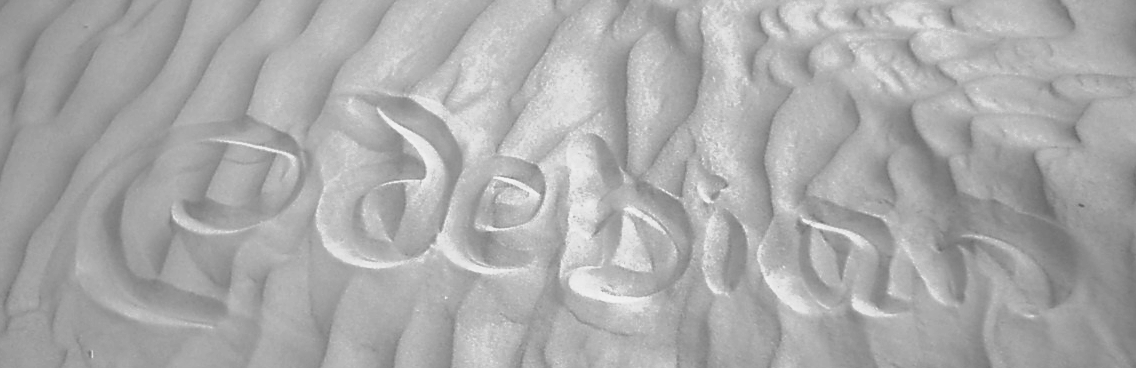
\includegraphics[width=16cm]{image2006-natsu/guruguru-sand-light.png}\\
\vspace{-5cm}
\begin{center}
\section{#1}
\end{center}
\hfill{}\colorbox{white}{#2}\hspace{3cm}\space\\
\vspace{1cm}
\hrule
\vspace{0.5mm}
\hrule
\vspace{1cm}
}

% for dancerj
\newcommand{\fgref}[1]{図\ref{#1}}
\newcommand{\tbref}[1]{表\ref{#1}}


\begin{document}

\begin{titlepage}

% 毎月変更する部分, 本文の末尾も修正することをわすれずに
\title{
 第18回 東京エリア Debian 勉強会\\事前資料}
\date{2006年7月15日}
\author{Debian勉強会会場係 上川 純一\thanks{Debian Project Official Developer}} 
\maketitle
\thispagestyle{empty}
\end{titlepage}

\newpage
\tableofcontents

\dancersection{Introduction To Debian 勉強会}{上川 純一}

今月のDebian勉強会へようこそ。
これからDebianのあやしい世界に入るという方も、すでにどっぷりとつかってい
るという方も、月に一回Debianについて語りませんか?

目的として下記の二つを考えています。

\begin{itemize}
 \item メールではよみとれない、もしくはよみとってられないような情報を情
       報共有する場をつくる
 \item まとまっていないDebianを利用する際の情報をまとめて、ある程度の塊と
       して出してみる
\end{itemize}

また、東京にはLinuxの勉強会はたくさんありますので、Debianに限定した勉強
会にします。Linuxの基本的な利用方法などが知りたい方は、他でがんばってくださ
い。
Debianの勉強会ということで究極的には参加者全員がDebian Packageを
がりがりと作りながらスーパーハッカーになれるような姿を妄想しています。

Debianをこれからどうするという能動的な展開への土台としての空間を提供し、
情報の共有をしたい、というのが目的です。
次回は違うこと言ってるかもしれませんが、御容赦を。

\subsection{講師紹介}

\begin{itemize}
 \item{岩松 信洋} 翻訳のインフラについて紹介します。
 \item{上川 純一} 宴会の幹事です。
\end{itemize}

\subsection{事前課題紹介}

今回の事前課題は
「今回実現すること」
というタイトルで200-800文字程度の文章を書いてください。
というものでした。
その課題に対して下記の内容を提出いただきました。

\subsubsection{岩松 信洋}

ジンギスカン食います。

\subsubsection{上川}

北海道の空気を吸います。

\dancersection{最近のDebian関連のミーティング報告}{上川 純一}

\subsection{東京エリアDebian勉強会17回目報告}
% (query-replace-regexp "<.*>" "")

東京エリアDebian勉強会報告。6月の第17回Debian勉強会を実施しました。岩松
さんがDebian Conference の報告をしました。上川が cowbuilder の使い方につ
いて発表しました。
	  
今回の参加人数は16人でした。
	  
最初は事前課題の発表。みなさん Debconf に参加するなら、裏方を手伝います、
という意見が多かったようです。岩松さんはFlashのBOFを開催するとのことで、
来年に期待です。

Debian weekly news quiz はあけどさんが満点をとりました。おめでとうござい
ます。小林さんは一問不正解だったようです。残念。
	  	  
岩松さんが Debconf について発表。セッションの紹介などをしました。
	  
上川が\texttt{pbuilder/cowdancer/cowbuilder}について発表しました。いかに
高速にしたのか、ということを発表しました。いままで、こんなに簡単なことを
するのに2分も待っていたのですね、ということに驚愕、よくみんな我慢してく
れた!と盛り上がりました。
	  
宴会は「いねや」にて開催。食事の量がすくなくて、最初に注文した商品が出終
るよりもはやくラストオーダーの時間が来たりといろいろと不手際がありました、
失礼しました。
	  
\dancersection{MacBook に Debian をインストール}{上川}
\label{dancerjmacbook}

Apple が2006年春に発売開始した Intel ベースのMacBook に MacOS X と Debian を
dual-boot でインストールの流れを紹介します。

MacOS X を削除してDebian のみをインストールする方法については、おそらく
liloをMBRから起動するように設定すれば最新ファームウェアは起動してくれま
すが、検証していません。

\subsection{インストール用にパーティション準備}

購入直後の状態では、Mac OS X が全部の領域を占めています。その MacOS X 
パーティションを縮小し、Debianがインストールできるようにします。Mac OS X
は20GB程度の領域を必要とするようですので、20GBまで縮小してしまいましょう。

diskutil resizevolume コマンドでボリュームサイズを動的に変更することがで
きます。\footnote{resizevolumeコマンドはMac OS X 10.4.6の機能拡張のようです。}

\begin{commandline}
Mac OS X $ df -h
Filesystem                Size   Used  Avail Capacity  Mounted on
/dev/disk0s2               74G    17G    57G    23%    /
devfs                      95K    95K     0B   100%    /dev
fdesc                     1.0K   1.0K     0B   100%    /dev
<volfs>                   512K   512K     0B   100%    /.vol
automount -nsl [171]        0B     0B     0B   100%    /Network
automount -fstab [179]      0B     0B     0B   100%    /automount/Servers
automount -static [179]     0B     0B     0B   100%    /automount/static
/dev/disk0s1              197M   512B   197M     0%    /efi

Mac OS X $ sudo diskutil resizevolume disk0s2 20G
Started resizing on disk disk0s2 Macintosh HD
Verifying

Resizing Volume
Adjusting Partitions

Finished resizing on disk disk0s2 Macintosh HD
WARNING: You must now reboot!

# diskutil list
/dev/disk0
   #:                   type name               size      identifier
   0:  GUID_partition_scheme                    *74.5 GB  disk0
   1:                    EFI                    200.0 MB  disk0s1
   2:              Apple_HFS Macintosh HD       20.0 GB   disk0s2

\end{commandline}

\subsection{rEFItのインストール}

rEFItはEFI専用ブートローダです。
rEFIt\footnote{\url{http://refit.sourceforge.net/} 執筆時点のバージョン
は0.7でした。} イメージを MacOS X にインストールします。インストールする
場所はどこでもよいのですが、ドキュメントに従ってみましょう。
\texttt{/efi} あたりにファイルを展開し、 rEFIt に含まれている、
\texttt{./enable.sh} を実行します。スクリプト内部で \texttt{bless} コマ
ンド\footnote{EFIでのOS起動優先順序を変更してくれるツール}を実行してくれ
ます。これで、起動時に自動で rEFIt が実行されるようになります。

DebianのrEFItパッケージを利用してインストールする場合にはバージョン0.7-3 
時点では enable.sh を提供していません、直接blessコマンドを入力してくださ
い。

\texttt{sudo bless --folder \textit{[refit.efiのあるディレクトリへのフルパス]} --file \textit{[refit.efiへのフルパス]}}

\begin{center}
  \includegraphics[width=0.5\hsize]{image200607/bootchain.ps}
\end{center}

\subsection{Debian のインストール}

2006年7月版以降のetch\footnote{これ以前については動作確認をしていません。} 
のインストーラを利用してインストールします。

CDROMから起動するためには、CDROMを挿入してから、Cを押しながら起動すれば
よいです。もしくは、option キーを押しながら起動するとファームウェアの選
択画面が起動します。rEFItのメニューからもCDROMからの起動を選択できます。
\footnote{2006年7月時点でDebian Installer で利用しているLinux カーネル 
2.6.15, 2.6.16 あたりでは Intel Mac に対応できていない問題があり、5回に
4回程度は「APICエラー」なるものが発生し、起動に失敗するので、根気よく起
動するまでがんばってください。2.6.17 以降ではIntel Mac 向けの修正が一部
マージされているので、状況は改善しています。}

パーティションを切る部分\footnote{注意事項としては、既存のEFI FATとMac
OS Xのパーティションは削除しないこと。LILOをインストールする予定のパーティ
ションはパーティション番号 3 か 4 にすること、ということがあります。5番
目以降のパーティションは MBRの制限があるので利用できません。}を過ぎ、パッ
ケージがインストールされたら、LILOをインストールする直前の部分まで実施し
ます。

この時点では LILO が現在動作できない状態になっています。\footnote{parted 
が GPT の仕様に準拠しており、partition 1 のみしかない MBR上のパーティショ
ンテーブルを再作成していることによるようです。}ここで、MBRをGPTに同期さ
せる作業を実施します。ここで、Alt-F2 で仮想コンソールを切替え、コマンド
ラインにうつります。gptsync コマンドを実行してください\footnote{今後はイ
ンストーラから実施できるように改善したいです}。 現状のインストール方法と
しては、\texttt{chroot /target bin/sh}としてインストール先の chrootに入
り、そこから \texttt{apt-get install refit} でパッケージをインストール、
そして\texttt{ gptsync} コマンドでGPTからMBRに同期させます。

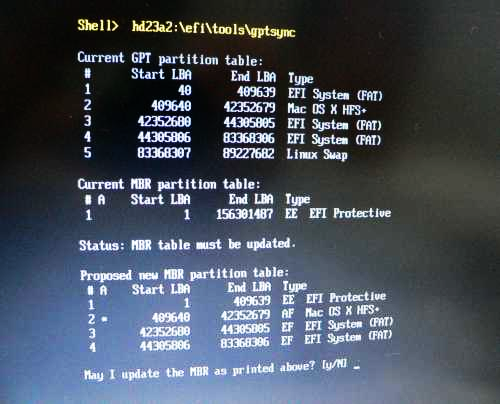
\includegraphics[width=0.9\hsize]{image200607/gptsync.png}

この状態で、インストーラの画面に Alt-F1で戻り、LILO を MBR ではなく、
Linux 用のパーティションにインストールします。再起動するとrEFItからLinux
を指定して起動できるようになっています。

\subsection{各種デバイスの設定}
\subsubsection{Xの設定}

\texttt{X} は \texttt{i810} ドライバで設定します。
\texttt{915resolution} パッケージをインストールします。
解像度は 1280x800 です。

\texttt{/etc/default/915resolution}の例です:\\
\begin{commandline}
#
# 915resolution default
#
# find free modes by  /usr/sbin/915resolution -l
# and set it to MODE
# e.g. use MODE=54 
MODE=32
#
# and set resolutions for the mode.
# e.g. use XRESO=1024 and YRESO=768
XRESO=1280
YRESO=800
#
# We can also set the pixel mode.
# e.g. use BIT=32
# Please note that this is optional,
# you can also leave this value blank.
BIT=
\end{commandline}

xorg.conf の例です\footnote{デフォルトで外部出力もするように設定してあります}:

\begin{commandline}
Section "Files"
	FontPath	"/usr/share/fonts/X11/misc"
	FontPath	"/usr/X11R6/lib/X11/fonts/misc"
	FontPath	"/usr/share/fonts/X11/cyrillic"
	FontPath	"/usr/X11R6/lib/X11/fonts/cyrillic"
	FontPath	"/usr/share/fonts/X11/100dpi/:unscaled"
	FontPath	"/usr/X11R6/lib/X11/fonts/100dpi/:unscaled"
	FontPath	"/usr/share/fonts/X11/75dpi/:unscaled"
	FontPath	"/usr/X11R6/lib/X11/fonts/75dpi/:unscaled"
	FontPath	"/usr/share/fonts/X11/Type1"
	FontPath	"/usr/X11R6/lib/X11/fonts/Type1"
	FontPath	"/usr/share/fonts/X11/100dpi"
	FontPath	"/usr/X11R6/lib/X11/fonts/100dpi"
	FontPath	"/usr/share/fonts/X11/75dpi"
	FontPath	"/usr/X11R6/lib/X11/fonts/75dpi"
	# path to defoma fonts
	FontPath	"/var/lib/defoma/x-ttcidfont-conf.d/dirs/TrueType"
EndSection

Section "Module"
	Load	"i2c"
	Load	"bitmap"
	Load	"ddc"
	Load	"dri"
	Load	"extmod"
	Load	"freetype"
	Load	"glx"
	Load	"int10"
	Load	"type1"
	Load	"vbe"
EndSection


Section "InputDevice"
	Identifier	"Generic Keyboard"
	Driver		"kbd"
	Option		"CoreKeyboard"
	Option		"XkbRules"	"xorg"
	Option		"XkbModel"	"pc104"
	Option		"XkbLayout"	"us"
	Option		"XkbOptions"	"ctrl:nocaps"
EndSection

Section "InputDevice"
	Identifier	"Configured Mouse"
	Driver		"mouse"
	Option		"CorePointer"
	Option		"Device"		"/dev/input/mice"
	Option		"Protocol"		"ExplorerPS/2"
	Option		"Emulate3Buttons"	"true"
EndSection

Section "InputDevice"
	Identifier	"Synaptics Touchpad"
	Driver		"synaptics"
	Option		"SendCoreEvents"	"true"
	Option		"Device"		"/dev/psaux"
	Option		"Protocol"		"auto-dev"
	Option		"HorizScrollDelta"	"0"
EndSection


Section "Device"
	Identifier	"Generic Video Card"
	Driver		"i810"
	Screen		0
	Option "MonitorLayout" "CRT,LFP"
	BusID		"PCI:0:2:0"
EndSection

Section "Device"
	Identifier	"Device1"
	Driver		"i810"
	Screen		1
	Option "MonitorLayout" "CRT,LFP"
	BusID		"PCI:0:2:0"
EndSection

\end{commandline}

続く

\begin{commandline}



Section "Monitor"
	Identifier	"Generic Monitor"
	Option		"DPMS"
	HorizSync	28-64
	VertRefresh	43-60
EndSection


Section "Monitor"
	Identifier	"External Monitor"
	Option		"DPMS"
	HorizSync	28-64
	VertRefresh	43-60
EndSection

Section "Screen"
	Identifier	"Default Screen"
	Device		"Generic Video Card"
	Monitor		"Generic Monitor"
	DefaultDepth	24
	SubSection "Display"
		Depth		1
		Modes		"1280x800" "1024x768" "800x600" "640x480"
	EndSubSection
	SubSection "Display"
		Depth		4
		Modes		"1280x800" "1024x768" "800x600" "640x480"
	EndSubSection
	SubSection "Display"
		Depth		8
		Modes		"1280x800" "1024x768" "800x600" "640x480"
	EndSubSection
	SubSection "Display"
		Depth		15
		Modes		"1280x800" "1024x768" "800x600" "640x480"
	EndSubSection
	SubSection "Display"
		Depth		16
		Modes		"1280x800" "1024x768" "800x600" "640x480"
	EndSubSection
	SubSection "Display"
		Depth		24
		Modes		"1280x800" "1024x768" "800x600" "640x480"
	EndSubSection
EndSection

Section "Screen"
	Identifier "Secondary Screen"
	Device "Device1"
	Monitor "External Monitor"
	DefaultDepth 24
	SubSection "Display"
		   Depth 1
		   Modes "1024x768" "800x600"
	EndSubSection
	SubSection "Display"
		   Depth 4
		   Modes "1024x768" "800x600"
	EndSubSection
	SubSection "Display"
		   Depth 8
		   Modes "1024x768" "800x600"
	EndSubSection
	SubSection "Display"
		   Depth 16
		   Modes "1024x768" "800x600"
	EndSubSection
	SubSection "Display"
		   Depth 24
		   Modes "1024x768" "800x600"
	EndSubSection
EndSection

Section "ServerLayout"
	Identifier "Dual-monitor Layout"
	Screen 0 "Default Screen"
	Screen 1 "Secondary Screen" LeftOf "Default Screen"
	# Option "Clone" "On"
	#Option "Xinerama" "On"
	InputDevice "Generic Keyboard"
	InputDevice "Configured Mouse"
	InputDevice "Synaptics Touchpad"
EndSection

Section "DRI"
	Mode	0666
EndSection
 
\end{commandline}

キーバインドは .xsession \footnote{最近はデフォルトでは .gnomerc とい
うファイルが使われるようです。 GDMからデフォルトのシステムセッションを明
示的に選択すれば .xsession を実行してくれるようです。}の中で次のような
設定をしています。右のappleキーを押すと全角・半角キーに割り当てられてい
ます。option と apple キーはよく押し間違えるので、両方を Alt\_Lとして設
定しています。また、イジェクトキーとキーボードの下の部分にあるENTERキー
をマウス用のキーとして定義しています。\footnote{xkbsetパッケージが必要}。
また、外部マウスをUSBで接続した場合も問題なく動作します。

\begin{commandline}
xmodmap -e "keycode 115 = Alt_L"
xmodmap -e "keycode 116 = Zenkaku_Hankaku" # right-apple
xmodmap -e "keycode 108 = Pointer_Button3" # KP-ENTER
xmodmap -e "keycode 204 = Pointer_Button2" # eject
xkbset m
\end{commandline}

\subsubsection{liloの設定}

いつもの癖でboot(/dev/sda3, ext2)とroot(/dev/sda4 ext3)をわけてしまっているのでちょっとややこ
しい例ですが、現在利用しているlilo.conf の例です:

\begin{commandline}
boot=/dev/sda3
root=/dev/sda4
map=/boot/map
delay=20
default=Linux-20060705

image=/boot/vmlinuz-2.6.17dancer-20060701
        label=Linux-20060701
        read-only

image=/boot/vmlinuz-2.6.17dancer
        label=Linux-20060705
        read-only

image=/vmlinuz
        label=Linux
        read-only

image=/vmlinuz.old
        label=LinuxOLD
        read-only
        optional
        initrd=/initrd.img.old

\end{commandline}


デフォルトでインストールされているカーネルが 2.6.17 以前のものであれば、
よく起動時にパニックをおこすので、Intel Mac 対応の 2.6.17 以降のものに
変更しましょう。

\subsubsection{サウンドカード設定}

サウンドカードは \texttt{snd\_hda\_intel} ドライバで対応できる ALSAのオーディオデ
バイスです。

\begin{commandline}
$ cat /proc/asound/cards
 0 [Intel          ]: HDA-Intel - HDA Intel
                      HDA Intel at 0x90440000 irq 50
\end{commandline}

\subsubsection{CPUの動的周波数設定}

cpufreq は \texttt{speedstep\_centrino} で動作します。
apt-get install cpufreqd でインストールして、cpufreqd を動作させてあげ
ると、動作します。

\subsubsection{USBの設定}

USBは UHCI, EHCI です。
通常は特に設定必要ないはずです。

\subsubsection{電源設定}

バッテリーはまともにサポートしているようです。
ただ、電源の全容量が出ていないので、gnomeから変なメッセージは出ました。

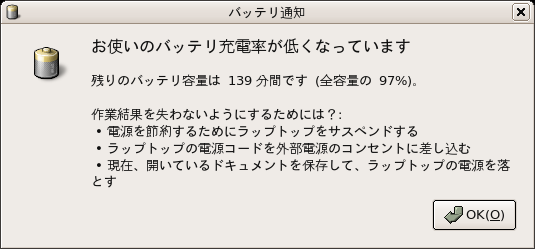
\includegraphics[width=0.8\hsize]{image200607/batterylo.png}

\subsubsection{ネットワークの設定}

有線ネットワークは SKY2 のドライバを利用します。

無線ネットワークは madwifi で対応できます。
インストール方法は下記です。

\begin{itemize}
  \item \texttt{sudo apt-get install madwifi-source madwifi-tools madwifi-doc}
  \item \texttt{sudo m-a prepare}
  \item \texttt{sudo m-a a-i madwifi}
  \item \texttt{sudo modprobe ath\_pci}
\end{itemize}

放っておくとhotplugにより、起動時に自動ロードされて有効になります。
\texttt{/etc/hotplug/blacklist.d/}にファイルを作成し、下記のような内容を
追加しておくと手動でロードしないと有効にならないようにできます。飛行機に
のる場合などのためには必要かもしれません。

\begin{commandline}
 ath_pci
\end{commandline}

以下、インストール字のログの例です。

\begin{commandline}
 $ sudo apt-get install madwifi-source madwifi-tools madwifi-doc
 $ sudo m-a prepare
Getting source for kernel version: 2.6.17dancer
/lib/modules/2.6.17dancer/source のカーネルヘッダを利用できます
symlink を作成中...
apt-get install build-essential
パッケージリストを読み込んでいます... 完了
依存関係ツリーを作成しています... 完了
以下のパッケージが新たにインストールされます:
  build-essential
アップグレード: 0 個、新規インストール: 1 個、削除: 0 個、保留: 94 個。
6916B のアーカイブを取得する必要があります。
展開後に追加で 20.5kB のディスク容量が消費されます。
取得:1 http://ftp.jp.debian.org sid/main build-essential 11.2 [6916B]
6916B を 0s で取得しました (81.0kB/s)
パッケージフィールドを読み込んでいます... 完了
パッケージ状態を読み込んでいます... 完了
バグレポートを取得しています... 完了
(データベースを読み込んでいます ... 現在 101852 個のファイルとディレクトリがインストールされています。)
(.../build-essential_11.2_i386.deb から) build-essential を展開しています...
build-essential (11.2) を設定しています ...

完了!
$ sudo m-a a-i madwifi
パッケージリストを読み込んでいます... 完了
依存関係ツリーを作成しています... 完了
madwifi-source はすでに最新バージョンです。
アップグレード: 0 個、新規インストール: 0 個、削除: 0 個、保留: 94 個。

1 パッケージについての情報を更新しました
Extracting the package tarball, /usr/src/madwifi.tar.bz2, please wait...
\end{commandline}

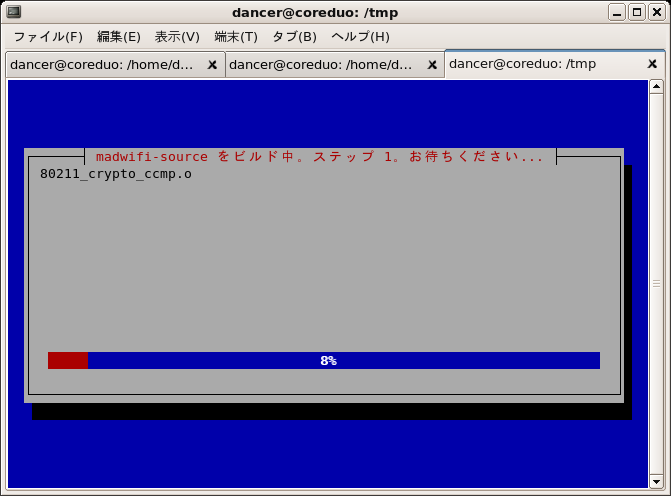
\includegraphics[width=0.8\hsize]{image200607/madwifi.png}

\begin{commandline}
/home/dancer/shared/git/madwifi-modules-2.6.17dancer_0.svnr1644.0.9.0-2+20060705_i386.deb が完了しました。
未選択パッケージ madwifi-modules-2.6.17dancer を選択しています。
(データベースを読み込んでいます ... 現在 101861 個のファイルとディレクトリがインストールされています。)
(.../madwifi-modules-2.6.17dancer_0.svnr1644.0.9.0-2+20060705_i386.deb から) madwifi-modules-2.6.17dancer 
を展開しています...
madwifi-modules-2.6.17dancer (0.svnr1644.0.9.0-2+20060705) を設定しています ...

$ sudo modprobe ath_pci
$ lsmod | grep ath_pci
ath_pci                82212  0
ath_rate_sample        11776  1 ath_pci
wlan                  167132  4 wlan_scan_sta,ath_pci,ath_rate_sample
ath_hal               192208  3 ath_pci,ath_rate_sample
$ dmesg | tail -20
eth1: no IPv6 routers present
ath_hal: module license 'Proprietary' taints kernel.
ath_hal: 0.9.17.2 (AR5210, AR5211, AR5212, RF5111, RF5112, RF2413, RF5413)
wlan: 0.8.4.2 (svn r)
ath_rate_sample: 1.2 (svn r)
ath_pci: 0.9.4.5 (svn r)
Device `[PXS2]is not power manageable<6>ACPI: PCI Interrupt 0000:02:00.0[A] -> GSI 17 (level, low) -> IRQ 169
PCI: Setting latency timer of device 0000:02:00.0 to 64
wifi0: 11a rates: 6Mbps 9Mbps 12Mbps 18Mbps 24Mbps 36Mbps 48Mbps 54Mbps
wifi0: 11b rates: 1Mbps 2Mbps 5.5Mbps 11Mbps
wifi0: 11g rates: 1Mbps 2Mbps 5.5Mbps 11Mbps 6Mbps 9Mbps 12Mbps 18Mbps 24Mbps 36Mbps 48Mbps 54Mbps
wifi0: H/W encryption support: WEP AES AES_CCM TKIP
wifi0: mac 10.3 phy 6.1 radio 10.2
wifi0: Use hw queue 1 for WME_AC_BE traffic
wifi0: Use hw queue 0 for WME_AC_BK traffic
wifi0: Use hw queue 2 for WME_AC_VI traffic
wifi0: Use hw queue 3 for WME_AC_VO traffic
wifi0: Use hw queue 8 for CAB traffic
wifi0: Use hw queue 9 for beacons
wifi0: Atheros 5424: mem=0x90100000, irq=169

$ /sbin/ifconfig ath0
ath0      リンク方法:イーサーネット  ハードウェアアドレス 00:16:CB:BA:76:E7 
          inetアドレス:192.168.22.42 ブロードキャスト:192.168.22.255 マスク:255.255.255.0
          inet6アドレス: fe80::216:cbff:feba:76e7/64 範囲:リンク
          UP BROADCAST RUNNING MULTICAST  MTU:1500  Metric:1
          RX packets:1176 errors:0 dropped:0 overruns:0 frame:0
          TX packets:1607 errors:0 dropped:0 overruns:0 carrier:0
      衝突(Collisions):0 TXキュー長:0 
          RX bytes:230678 (225.2 KiB)  TX bytes:1306390 (1.2 MiB)

\end{commandline}




\subsubsection{リモコン}

赤外線のリモコンは使えるようです。カーネル用のデバイスドライバが存在しま
す。2.6.18以降にとりこまれるのではないでしょうか?
ユーザ空間で利用できるドライバは作成しておきました。
\footnote{\url{http://www.netfort.gr.jp/~dancer/diary/daily/2006-Jul-12.html.ja}}

\subsubsection{iSight}

iSight は linux-uvcデバイスです。
ファームウェアのロードが必要です。
次の手順でインストールができます。

\begin{itemize}
 \item \texttt{apt-get install linux-uvc-tools linux-uvc-source}
 \item \texttt{module-assistant auto-install linux-uvc}
\end{itemize}

アプリケーションはekigaなどを利用しましょう。
v4l2デバイスなので、v4l2対応のソフトウェアが必要です。

\begin{itemize}
 \item \texttt{apt-get install ekiga libpt-plugins-v4l2}
\end{itemize}

実際にロードするには、Mac OS Xのデバイスドライバに入っているファームウェ
アをロードしてからモジュールをロードします。ドライバのある場所のディレク
トリ階層が深いので注意。

\begin{itemize}
 \item \texttt{sudo mount /dev/sda2 /mnt/macosx}
 \item \texttt{sudo macbook-isight-firmware-loader
       /mnt/mac/System/Library/Extensions/IOUSBFamily.kext/Contents/PlugIns
       /AppleUSBVideoSupport.kext/Contents/MacOS/AppleUSBVideoSupport}
 \item \texttt{modprobe uvcvideo}
\end{itemize}


\subsubsection{未確認のデバイス、手法}

Debianを自動起動させる方法がわかりません、rEFItはデフォルトでは、MacOSX
もしくはeLILOを起動しようとしてしまいます。eLILOを起動すると起動できない。
優先度の変更はどうやったらよいのか、というのがいまいち不明です。

サスペンドの方法。

スリープの方法。

CD-Rの動作はまだ確認していません。PATAパッチが必要という噂です。

\begin{commandline}
 
 # cdrecord -scanbus
 scsibus0:
        0,0,0     0) *
        0,1,0     1) 'ATA     ' 'ST98823AS       ' '7.01' Disk
        0,2,0     2) *
        0,3,0     3) *
        0,4,0     4) *
        0,5,0     5) *
        0,6,0     6) *
        0,7,0     7) *
\end{commandline}

バックライトの制御ができるドライバは作成されているので、2.6.18か19くらい
には入るのではないでしょうか。

bluetoothについては未調査。

\subsection{発表履歴}

本資料は下記の場所での発表資料として作成されたものです。
内容については随時更新しながら、いくつかの場所で発表しています。

\begin{itemize}
 \item 2006年7月2日 秋葉原、CodeFestAkihabara  2006: 最終報告
 \item 2006年7月6日 恵比寿、SGIホール、カーネル読書会: mixi.jp の話の前座
 \item 2006年7月15日 北海道、OSC-Do 2006: 「Debian勉強会」のセッション
 \item 2006年7月29日 日々谷、TLUG: 「MacBookにMac OS XとDebianを
       dual-bootでインストール」
\end{itemize}

\subsection{参考文献}

ファームウェアの bootcamp まわりの開発の影響で、ほとんどのweb上の手順を
書いてある文献は現在の時点で手順が古くなっているので、参考にならない場合
が多いですが、今後更新されるかもしれません。

\begin{itemize}
 \item MacBook Developer Note: MacBookの論理構成図、ハードウェアの概観が解説されています。 
       \url{http://developer.apple.com/documentation/HardwareDrivers/Conceptual/MacBook_0605/index.html}
 \item 赤外線リモートコントロール用、IR Receiver パッチ
       \url{http://sourceforge.net/mailarchive/message.php?msg_id=16309282}
       \url{http://www.madingley.org/macmini/kernel/ir.patch}
 \item 赤外線リモートコントロールでXPDFプレゼンテーションするパッチ。
       \url{http://www.netfort.gr.jp/~dancer/diary/daily/2006-Jul-12.html.ja#2006-Jul-12-00:00:06}
 \item MacBook の仕様: 簡単に概要だけが説明されています。
       \url{http://support.apple.com/specs/macbook/macbook.html}
 \item iSight (IEEE1394 外部デバイス)のプログラミングガイド 
       \url{http://developer.apple.com/documentation/Hardware/Conceptual/iSightProgGuide/
iSightProgGuide.pdf}
 \item bluetooth のドキュメント: \url{http://developer.apple.com/documentation/HardwareDrivers/Conceptual/HWTech_Bluetooth/index.html#//apple_ref/doc/uid/TP40003032}
 \item mactel linuxのページ \url{http://mactel-linux.org/}、
       ここからたどれるメーリングリストで有用な情報が交換されています。
 \item rEFItのページ \url{http://refit.sourceforge.net/}
 \item \url{http://sharealike.org/index.php?m=200605}
 \item バックライト制御
       \url{http://modular.math.washington.edu/macbook/backlight/}
 \item Ubuntuのインストールについてのまとめページ
       \url{http://desrt.mcmaster.ca/macbook.xhtml}
 \item Gentoo の情報ページ 
       \url{http://gentoo-wiki.com/HARDWARE_Apple_MacBook}
 \item MadWifi Wiki
       \url{http://madwifi.org/wiki/UserDocs/Distro/Debian/MadWifing}
 \item Macbook Pro build-in iSight
       \url{http://blogs.gnome.org/view/rbultje/2006/07/08/0}
 \item linux usb video class, linux-uvc
       \url{http://linux-uvc.berlios.de}
 \item Debian wiki MacBook \url{http://wiki.debian.org/MacBook}
\end{itemize}

\dancersection{次回}{}

未定です。
内容は本日決定予定です。

参加者募集はまた後程。

\newpage

\vspace*{15cm}
\hrule
\vspace{2mm}

\includegraphics[width=2cm]{image200502/openlogo-nd.eps}
\noindent \Large \bf Debian 勉強会資料\\ \\
\noindent \normalfont 2006年7月15日 \hspace{5mm}  初版第1刷発行\\
\noindent \normalfont 東京エリア Debian 勉強会 (編集・印刷・発行)\\
\hrule

\end{document}
